\begin{figure*}[t!]
	\centering
	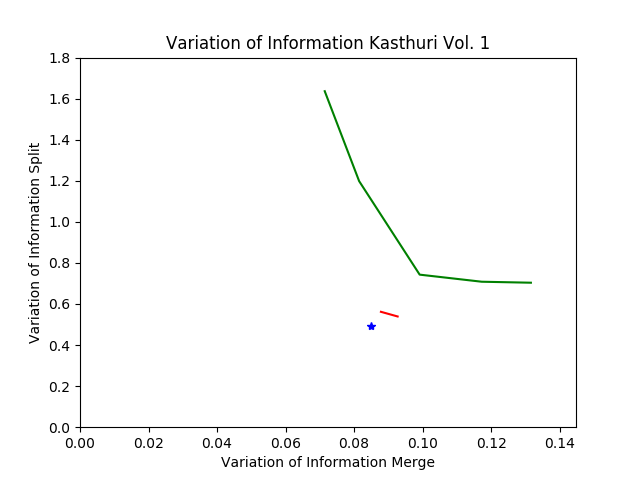
\includegraphics[width=0.23\linewidth]{./figures/variation_of_information-microns-train-600.png}
	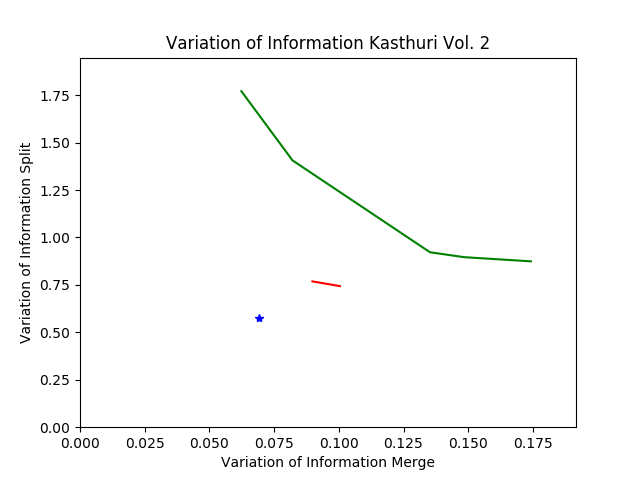
\includegraphics[width=0.23\linewidth]{./figures/variation_of_information-microns-test-600.png}
	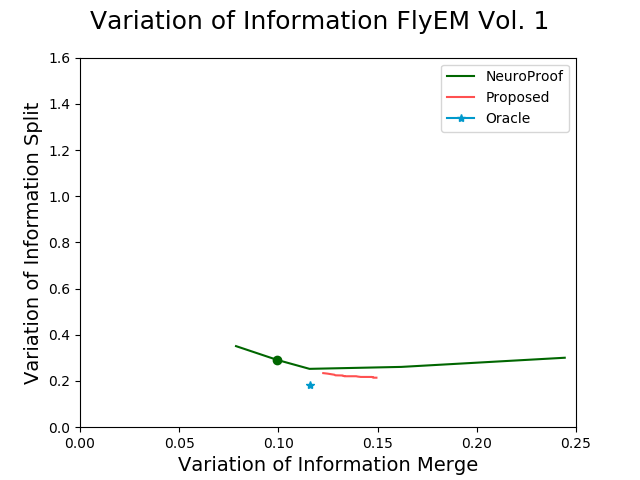
\includegraphics[width=0.23\linewidth]{./figures/variation_of_information-FlyEM-train-600.png}
	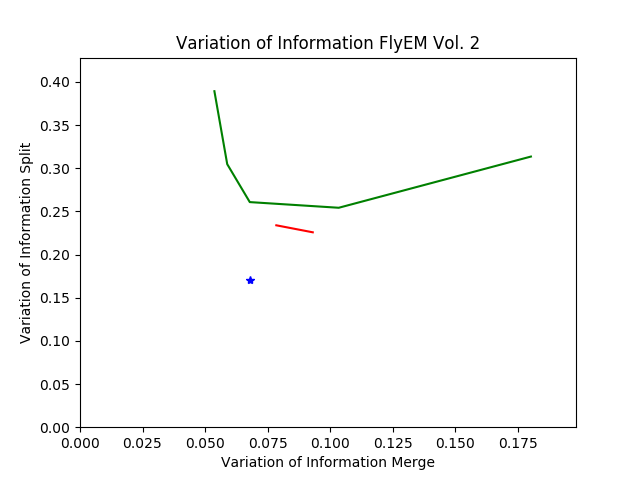
\includegraphics[width=0.23\linewidth]{./figures/variation_of_information-FlyEM-test-600.png}
	\caption{Our improvement (reD) on variation of information from the baseline NeuroProof segmentation (green). The blue dot represents an oracle which correctly partitions the graph.}
	\label{fig:variation-of-information}
\end{figure*}

\section{Results}

\subsection{Variation of Information Improvement}

We compute the variation of information for our segmentations against the expert-labeled ground truth datasets. 
The input segmentation to our network serves as a baseline. 
We evaluate NeuroProof (our input) at several different thresholds to create a variation of information curve. 
Figure \ref{fig:variation-of-information} shows the results on the datasets compared to the baseline (green) and an oracle (blue). 
The oracles sees the graph from our algorithm and correctly partitions the graph based on the ground truth. 
%TODO{Our methods decreases the split variation of information by a factor of XX\% and only increases the merge variation of information by a factor of XX\% on the test datasets.}
Figure \ref{fig:positive-results} shows some successful merges on the Kasthuri Vol. 2. 
Several of these successful examples combine multiple consecutive segments. 
The third example shows the correction of an oversegmented dendrite. 
Figure \ref{fig:negative-results} shows some errors made. 
In two of these examples the algorithm correctly predicted several merges but made just one error.
In the third example, an error in the initial segmentation propagated in our pipeline. 
In the next three subsections we show how each step in the pipeline contributes to this final result.

\begin{figure}[t]
	\centering
	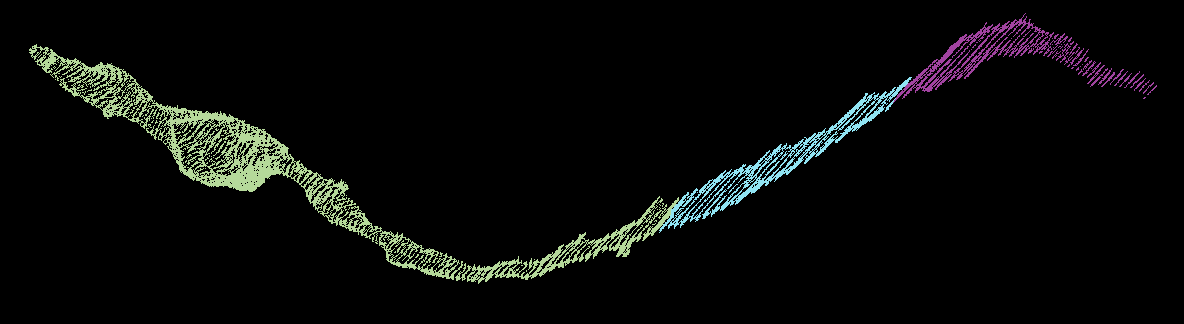
\includegraphics[width=0.85\linewidth]{./figures/multicut-correct1.png}
	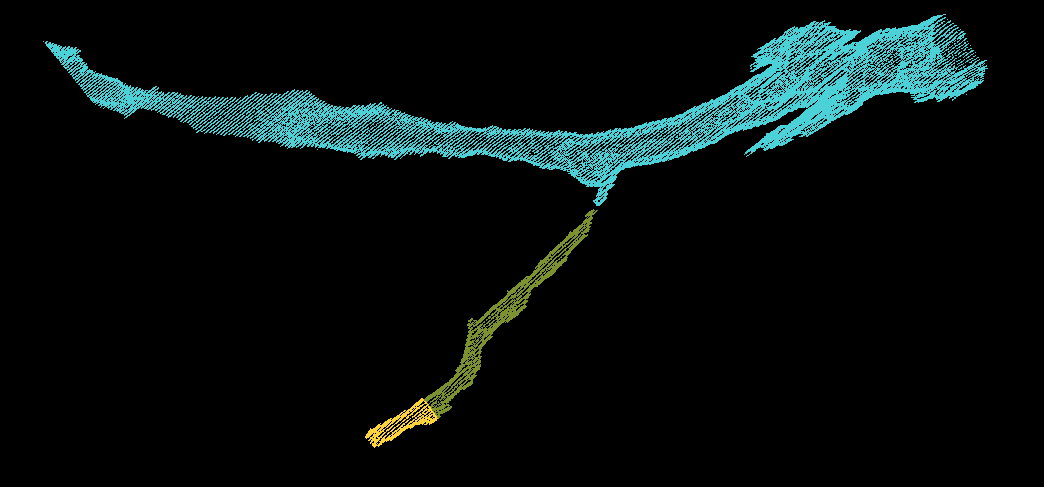
\includegraphics[width=0.85\linewidth]{./figures/multicut-correct2.png}
	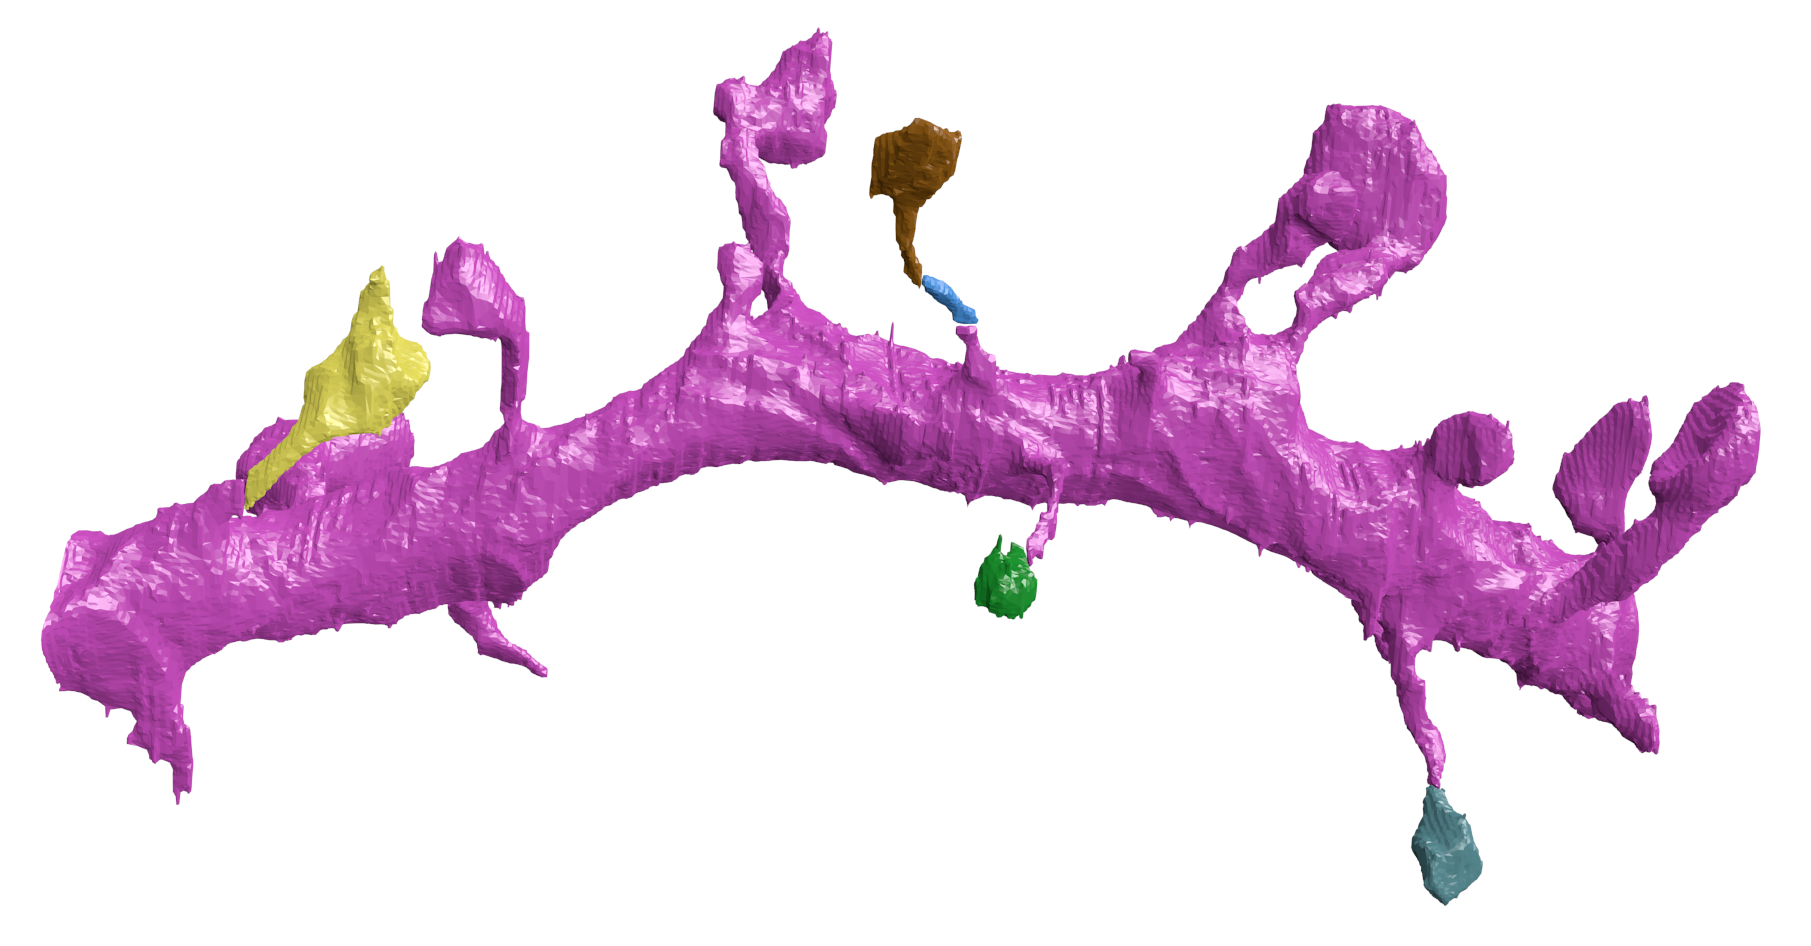
\includegraphics[width=0.85\linewidth]{./figures/multicut-correct3.png}
	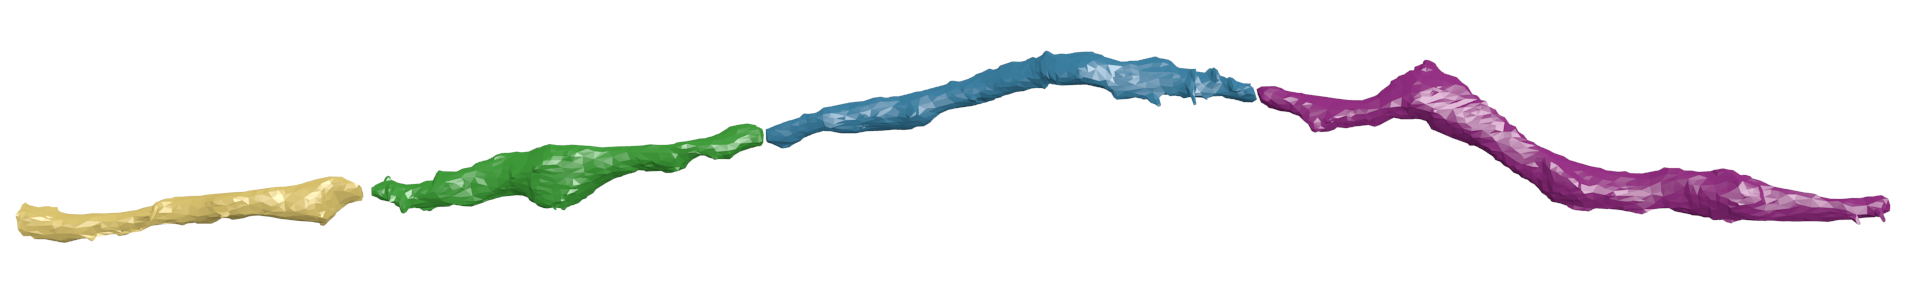
\includegraphics[width=0.85\linewidth]{./figures/multicut-correct4.png}
	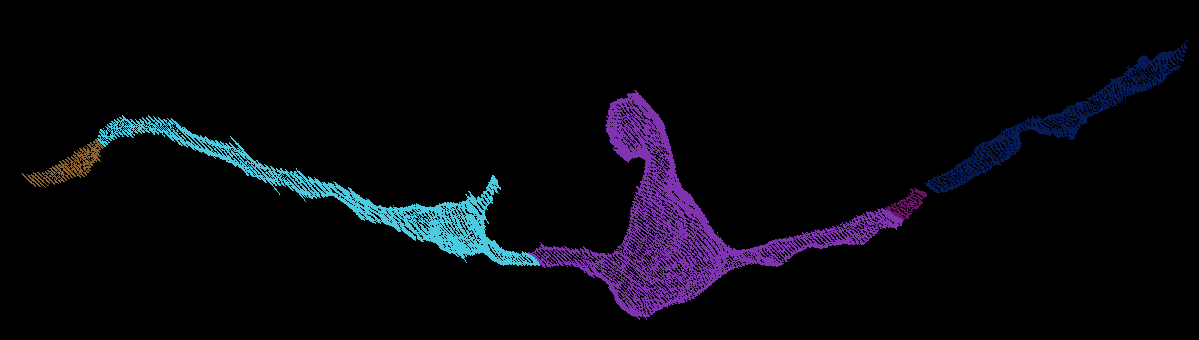
\includegraphics[width=0.85\linewidth]{./figures/multicut-correct5.png}
	\caption{Some correctly predicted results from our framework.}
	\label{fig:positive-results}
\end{figure}

\begin{figure}[t]
	\centering
	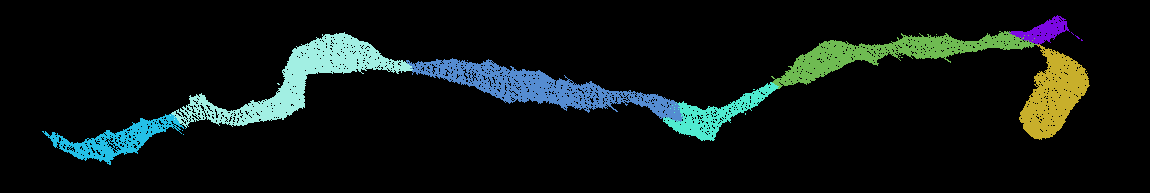
\includegraphics[width=0.85\linewidth]{./figures/multicut-incorrect1.png}
	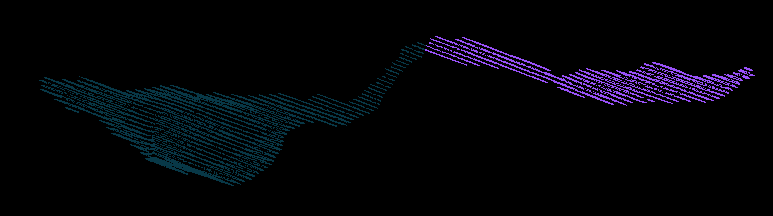
\includegraphics[width=0.85\linewidth]{./figures/multicut-incorrect2.png}
	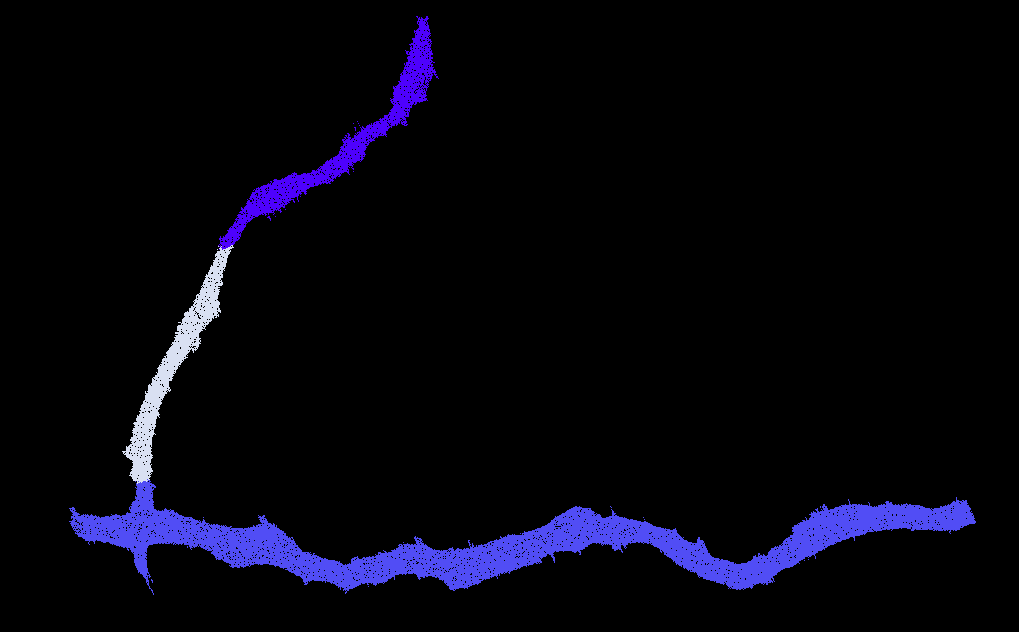
\includegraphics[width=0.85\linewidth]{./figures/multicut-incorrect3.png}
	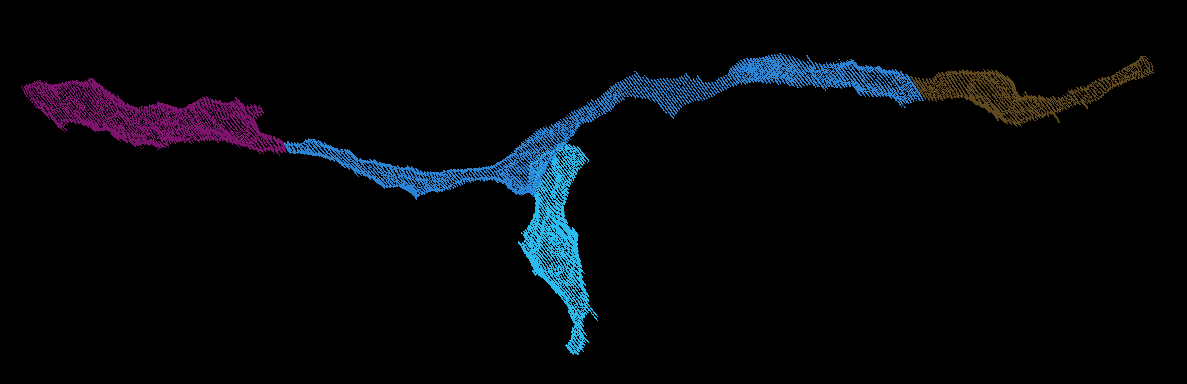
\includegraphics[width=0.85\linewidth]{./figures/multicut-incorrect4.png}
	\caption{Mistakes made by the proposed framework.}
	\label{fig:negative-results}
\end{figure}


\subsection{Pruning via Skeletonization}

\begin{table}
	\centering
	\small
	\begin{tabular}{c c c} \hline
		\textbf{Dataset} & \textbf{Baseline} & \textbf{After Pruning} \\ \hline
		Kasthuri Vol. 1 & 763 / 21242 (3.47\%) & 753 / 3459 (17.88\%) \\
		Kasthuri Vol. 2 & 1010 / 26073 (3.73\%) & 904 / 4327 (17.28\%) \\
		FlyEM Vol. 1 & 269 / 14875 (1.78\%) & 262 / 946 (21.69\%) \\
		FlyEM Vol. 2 & 270 / 16808 (1.58\%) & 285 / 768 (27.07\%)\\ \hline
	\end{tabular}
	\caption{The results of our pruning heuristic compared to the current baseline.}
	\label{table:skeletonization}
\end{table}

Table \ref{table:skeletonization} shows the results of pruning using the skeletonization heuristic.
The baseline algorithm considers all adjacent regions for merging. 
Our method removes a significant portion of these candidates while maintaining a large number of the true merge locations.
This edge pruning is essential for the graph partitioning algorithm which has a computational complexity dependence on the number of edges. 
Our pruning heuristic removes at least $6\times$ the number of edges between correctly split segments on all datasets, achieving a maximum removal ratio of $20\times$. 
Equally important is the number of split errors that remain after pruning.
These are the locations that we want to merge to create a more accurate reconstruction.
For every dataset, the number of positive candidates remains relatively even. 
However, since our heuristic does not enforce an adjacency constraint of two regions when constructing edges in the graph, the difference does not indicate the number of examples excluded by pruning. 
In fact, our method finds a number of examples which are non-adjacent.
Figure \ref{fig:skeleton-results} shows two example segments which are split errors.
The top example our algorithm missed but the segments are adjacent. 
The bottom example our algorithm found despite the fact that they are not adjacent.

\begin{figure}[h!]
	\centering
	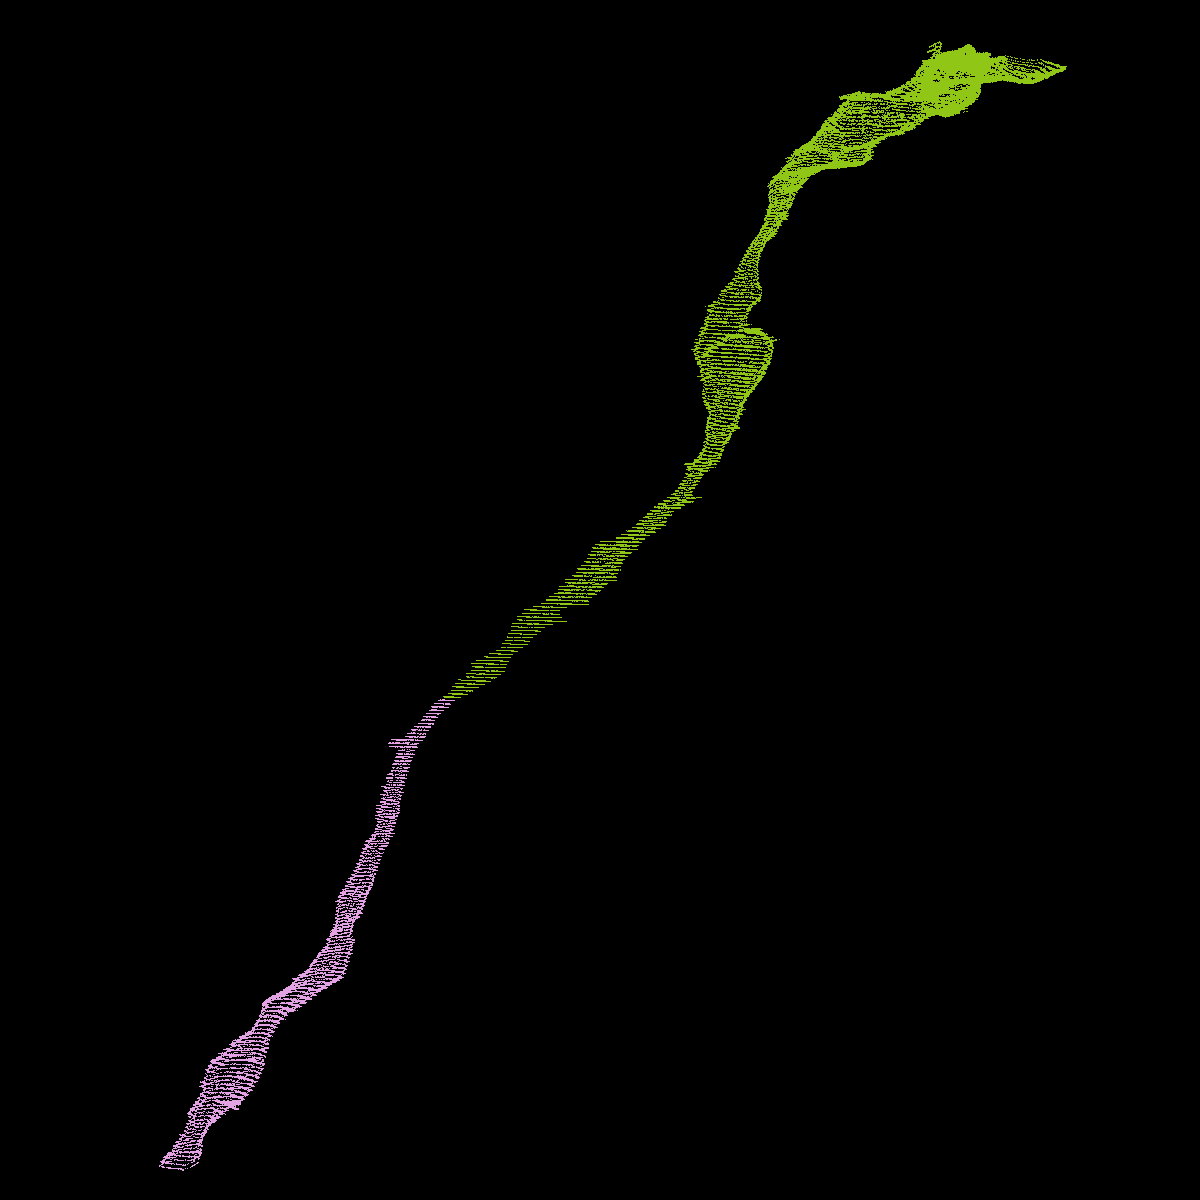
\includegraphics[width=0.85\linewidth]{./figures/merge_candidate1.png}
	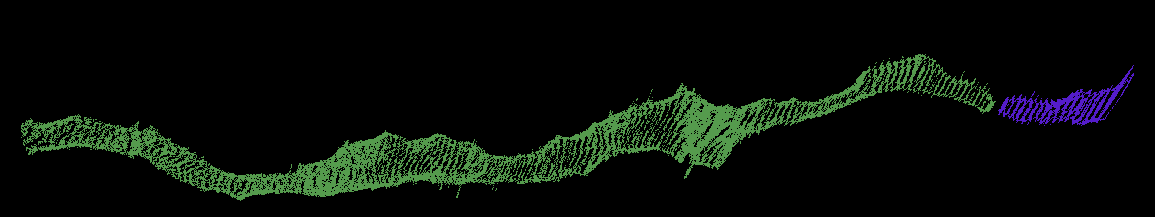
\includegraphics[width=0.85\linewidth]{./figures/merge_candidate2.png}
	\caption{Example merge candidates.}
	\label{fig:skeleton-results}
\end{figure}


\subsection{Classification Performance}

Table \ref{table:classification} shows the precision and recall for all of the datasets. 
Since, our method does not rely on the image data, we can train the network on an anisotropic dataset and get impressive results on an isotropic dataset. 

\begin{table}[h]
	\centering
	\begin{tabular}{c c c c} \hline
		\textbf{Dataset} & \textbf{Precision} & \textbf{Recall} & \textbf{Accuracy} \\ \hline
		Kasthuri Training & 0.919 & 0.936 & 0.974 \\
		Kasthuri Testing & 0.737 & 0.717 & 0.907 \\
		FlyEM Vol. 1 & 0.796 & 0.478 & 0.862 \\ 
		FlyEM Vol. 2 & 0.762 & 0.422 & 0.810 \\ \hline
	\end{tabular}
	\caption{Precision and recall for the training and three test datasets.}
	\label{table:classification}
\end{table}

\subsection{Graph Based Strategies}

Applying a graph-based optimization strategy increases the accuracy over the CNN alone. 
In our test datasets, we note an increase in precision on all datasets. 
For our segmentation problems we prefer a higher precision since it is more difficult to correct merge-errors. 
Table \ref{table:multicut} shows the changes in precision, recall, and accuracy for all three datasets in relation to the CNN.

\begin{table}[h]
	\centering
	\begin{tabular}{c c c c} \hline
		\textbf{Dataset} & $\Delta$ \textbf{Precision} & $\Delta$ \textbf{Recall} & $\Delta$ \textbf{Accuracy} \\ \hline
		Kasthuri Training & +3.60\% & -0.01\% & +0.60\% \\
		Kasthuri Testing & +7.59\% & -1.77\% & +1.38\% \\
		FlyEM Vol. 1 & +2.68\% & +0.76\% & +0.66\% \\ 
		FlyEM Vol. 2 & +2.22\% & -1.05\% & +0.29\% \\ \hline
	\end{tabular}
	\caption{Precision and recall for the training and three test datasets.}
	\label{table:multicut}
\end{table}


